\documentclass[ 12pt ]{article}

\usepackage{amsmath}
\usepackage{amssymb}
\usepackage{cancel}
\usepackage{tikz}
\usepackage{listings}
\usepackage{mathdots}
\usepackage[margin=.75in]{geometry}

\begin{document}

% title page
\title{%
	Homework 3 \\
	\large CS 477 Analysis of Algorithims \\
	Section 1001}
\author{Landon Fox}
\date{February 20, 2020}
\maketitle
\newpage

\begin{itemize}

	% problem 1
	\item[] {1) \large}
	\begin{itemize}

		% problem 1a
		\item[] 1a)
		The algorithim determines if the array has only unique elements.

		% problem 1b
		\item[] 1b)
		\begin{flalign}
			T(n) &= c_1(n - 1) + c_2 \sum_{i=0}^{n-2}(n-i) + c_3 \sum_{i=0}^{n-2}(n-i-1) + c_4 \nonumber \\
			&= c_4 + c_1(n - 1) - c_3(n - 1) + (c_2 + c_3) \sum_{i=0}^{n-2}(n - i) \nonumber \\
			&= \Theta(n) + (c_2 + c_3)(n(n - 1) - \frac{1}{2}(n - 1)(n - 2)) \nonumber \\
			&= \Theta(n) + (c_2 + C_3)(\frac{1}{2}n^2 + \frac{1}{2}n - 1) \nonumber \\
			T(n) &= \Theta(n^2) \nonumber
		\end{flalign}

	\end{itemize}

	% problem 2
	\item[] {2) \large}
	\begin{itemize}
		% problem 2a
		\item[] 2a)
		\begin{lstlisting}[language=C++]
    int largest( int* array, int start, int end )
    {
        if ( start == end )
            return start;
        int mid = ( start + end ) / 2;
        int left = largest( array, start, mid );
        int right = largest( array, mid + 1, end );
        if ( array[ left ] > array[ right ] )
            return left;
        return right;
    }
		\end{lstlisting}
		Program output:
		\begin{lstlisting}
    > Largest item of { 1, 4, 9, 3, 4, 9, 5, 6, 9, 3, 7 } is index:
    > 8
		\end{lstlisting}
		\newpage
		Program Demonstration: \\
		Divide:
		\begin{center}
			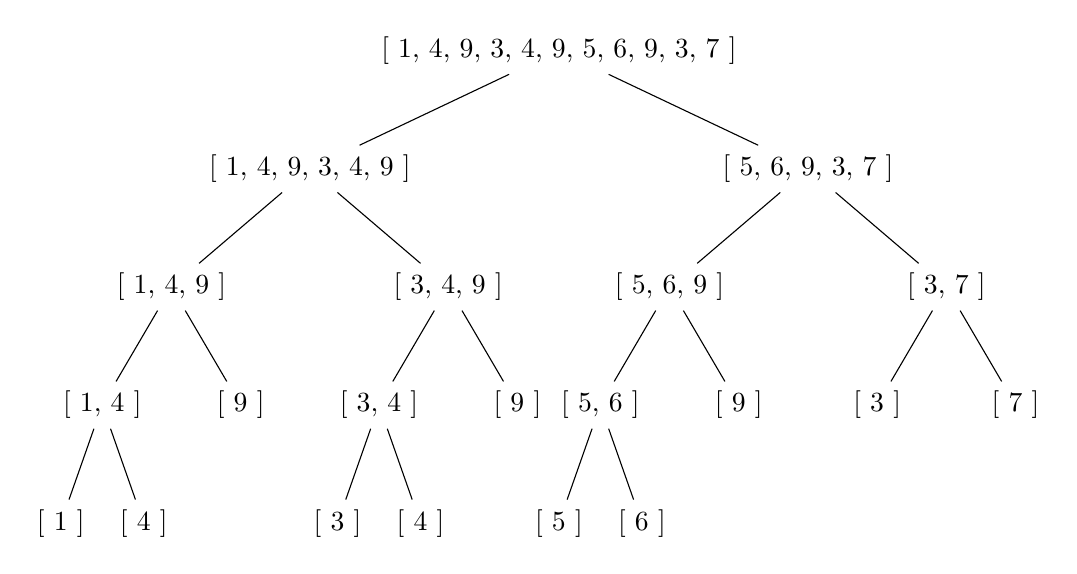
\begin{tikzpicture}[%
				level 1/.style={sibling distance=18em},
			  	level 2/.style={sibling distance=10em},
			  	level 3/.style={sibling distance=5em},
			  	level 4/.style={sibling distance=3em},
			  	every node/.style = {align=center,
			    top color=white, bottom color=white!20}]]
			  	\node {[ 1, 4, 9, 3, 4, 9, 5, 6, 9, 3, 7 ]}
					child { node {[ 1, 4, 9, 3, 4, 9 ]}
						child { node {[ 1, 4, 9 ]}
							child { node {[ 1, 4 ]}
								child { node {[ 1 ]} }
								child { node {[ 4 ]} }
							}
							child { node {[ 9 ]} }
						}
						child { node {[ 3, 4, 9 ]}
							child { node {[ 3, 4 ]}
								child { node {[ 3 ]} }
								child { node {[ 4 ]} }
							}
							child { node {[ 9 ]} }
						}
					}
					child { node {[ 5, 6, 9, 3, 7 ]}
						child { node {[ 5, 6, 9 ]}
							child { node {[ 5, 6 ]}
								child { node {[ 5 ]} }
								child { node {[ 6 ]} }
							}
							child { node {[ 9 ]} }
						}
						child { node {[ 3, 7 ]}
							child { node {[ 3 ]} }
							child { node {[ 7 ]} }
						}
					};
			\end{tikzpicture}
		\end{center}
		Conqure:
		\begin{center}
			\begin{tikzpicture}[%
				level 1/.style={sibling distance=18em},
			  	level 2/.style={sibling distance=10em},
			  	level 3/.style={sibling distance=5em},
			  	level 4/.style={sibling distance=3em},
			  	every node/.style = {align=center,
			    top color=white, bottom color=white!20}]]
			  	\node {[ 9 ]}
					child { node {$\cancel{[ 9 ]}$}
						child { node {$\cancel{[ 9 ]}$}
							child { node {$\cancel{[ 4 ]}$}
								child { node {$\cancel{[ 1 ]}$} }
								child { node {[ 4 ]} }
							}
							child { node {[ 9 ]} }
						}
						child { node {[ 9 ]}
							child { node {$\cancel{[ 4 ]}$}
								child { node {$\cancel{[ 3 ]}$} }
								child { node {[ 4 ]} }
							}
							child { node {[ 9 ]} }
						}
					}
					child { node {[ 9 ]}
						child { node {[ 9 ]}
							child { node {$\cancel{[ 6 ]}$}
								child { node {$\cancel{[ 5 ]}$} }
								child { node {[ 6 ]} }
							}
							child { node {[ 9 ]} }
						}
						child { node {$\cancel{[ 7 ]}$}
							child { node {$\cancel{[ 3 ]}$} }
							child { node {[ 7 ]} }
						}
					};
			\end{tikzpicture}
		\end{center}

		% problem 2b
		\item[] 2b)
		The algorithm will always favor the greatest index. In other words, the greatest value furthest to the right will always be chosen.
		In the provided array, index 8 will be returned.
		\newpage

		% problem 2c
		\item[] 2c)
		Solve:
		\begin{flalign}
			T(n) = c + 2T(\frac{n}{2})
		\end{flalign}
		Master's Method:
		\begin{flalign}
			a &= 2 \nonumber \\ 
			b &= 2 \nonumber \\
			f(n) &= c \nonumber \\
			g(n) &= n^{log_22} \nonumber \\
			&= n \nonumber \\
		\end{flalign}
		Case 1:
		\begin{flalign}
			c &\leq dn \nonumber \\
			f(n) &\leq dg(n) \nonumber \\
			\therefore T(n) &= \Theta(n) \nonumber
		\end{flalign}
	\end{itemize}

	% problem 3
	\item[] {3) \large}
	\begin{lstlisting}[language=C++]
    void arrange_sign( int* array, int n )
    {
        int k = 0;
        for ( int i = 0; i < n; ++i )
        {
            if ( array[ i ] < 0 )
            {
                int tmp = array[ k ];
                array[ k ] = array[ i ];
                array[ i ] = tmp;
                k++;
            }
        }
    }
	\end{lstlisting}
	Program output:
	\begin{lstlisting}
    > Arrange signs of { 4, -3, 9, 8, 7, -4, -2, -1, 0, 6, -5 }:
    > { -3, -4, -2, -1, -5, 4, 9, 8, 0, 6, 7 }
	\end{lstlisting}
	Program Demonstration:
	\begin{flalign}
		i=0,\; &[ 4, -3, 9, 8, 7, -4, -2, -1, 0, 6, -5 ] \nonumber \\
		i=2,\; &[ -3, 4, 9, 8, 7, -4, -2, -1, 0, 6, -5 ] \nonumber \\
		i=6,\; &[ -3, -4, 9, 8, 7, 4, -2, -1, 0, 6, -5 ] \nonumber \\
		i=7,\; &[ -3, -4, -2, 8, 7, 4, 9, -1, 0, 6, -5 ] \nonumber \\
		i=8,\; &[ -3, -4, -2, -1, 7, 4, 9, 8, 0, 6, -5 ] \nonumber \\
		i=11,\; &[ -3, -4, -2, -1, -5, 4, 9, 8, 0, 6, 7 ] \nonumber
	\end{flalign}

	% problem 4
	\item[] {4) \large}
	Binary Search and Sequential Search give the following complexities respectively:
	\begin{flalign}
		T_{bs}(n) &= c_1 + T(\frac{n}{2}) = clgn \nonumber \\
		T_{ss}(n) &= c_1 + c_2n \nonumber
	\end{flalign}
	The average binary search will always reach the bottom of the tree, as a result yielding the height of the tree.
	The average sequential searach will be in the middle of the array giving one half of the overall complexity.
	\begin{flalign}
		T_{bs,avg}(n) &= lgn \nonumber \\
		T_{ss,avg}(n) &= \frac{1}{2}n \nonumber
	\end{flalign}
	\begin{flalign}
		\frac{T_{ss,avg}(100000)}{T_{bs,avg}(100000)} &= \frac{\frac{1}{2}100000}{lg100000} \nonumber \\
		&\approx 3010 \nonumber
	\end{flalign}
	The average search of binary search is roughly 3010 times faster than sequential search.

	% problem 5
	\item[] {5) \large}
	To use binary search to conduct range searching, the algorithm will: \\
	First determine if the upper or lower bounds lie within the array by testing if the first element of the sorted array is greater than or equal to the lower bound
	and similiarly see if the upper bound is less than or equal than the last element. \\
	Second you must use binary search to find the lower and upper bound indicies within the array. If the indicies are found, the two values act as the inclusive bounds of
	your answer. Otherwise, values closest to the bounds must be found if they suffice. \\
	The worst case efficiency of this algorithim lies within the bounds not explicitly being found. It may take up to O(nlgn) time complexity just to find one value desireable 
	to the respective bound.

\end{itemize}

\end{document}
